\documentclass[12pt,a4paper]{article}
\usepackage[utf8]{inputenc}
\usepackage[margin=1in]{geometry}
\usepackage{graphicx}
\usepackage{xcolor}
\usepackage{tikz}
\usepackage{fontspec}

% Colors
\definecolor{phoenixorange}{RGB}{255,140,0}
\definecolor{phoenixgold}{RGB}{255,215,0}
\definecolor{codexblue}{RGB}{30,60,90}

\pagestyle{empty}

\begin{document}

\begin{titlepage}
\begin{center}

% Top decoration

\begin{tikzpicture}
\draw[line width=2pt, phoenixorange] (0,0) -- (15,0);
\end{tikzpicture}

\vspace{1cm}

% Title with fire emoji replacement
{\fontsize{48}{60}\selectfont\textcolor{phoenixorange}{\textbf{Phoenix 2.0}}}

\vspace{0.5cm}

{\fontsize{32}{40}\selectfont\textcolor{codexblue}{\textbf{Apex Edition}}}

\vspace{2cm}

% Symbolic representation
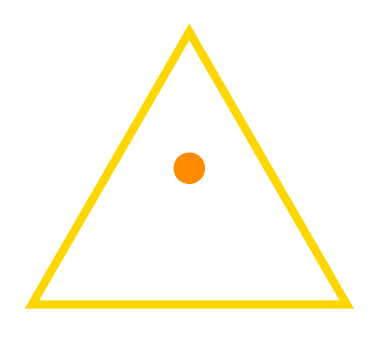
\begin{tikzpicture}
% Draw triangle (Apex symbol)
\draw[line width=3pt, phoenixgold] (0,0) -- (2,3.464) -- (4,0) -- cycle;
% Draw center dot (Kernel)
\fill[phoenixorange] (2,1.732) circle (0.2);
\end{tikzpicture}

\vspace{2cm}

% Subtitle
{\fontsize{24}{30}\selectfont\textcolor{codexblue}{\textbf{The Sovereign Kernel}}}

\vspace{0.5cm}

{\fontsize{20}{25}\selectfont\textcolor{codexblue}{Codex Documentation}}

\vspace{3cm}

% Version info

\begin{tikzpicture}
\draw[line width=1pt, phoenixorange] (0,0) -- (12,0);
\end{tikzpicture}

\vspace{0.5cm}

{\Large\textbf{Version 1.0.0}}

\vspace{0.3cm}

{\large The Sovereign Kernel Release}

\vspace{0.5cm}


\begin{tikzpicture}
\draw[line width=1pt, phoenixorange] (0,0) -- (12,0);
\end{tikzpicture}

\vfill

% Footer
{\large Phoenix--Hydrogenesi Codex}

\vspace{0.3cm}

{\normalsize 2024}

\vspace{0.5cm}

% Bottom decoration

\begin{tikzpicture}
\draw[line width=2pt, phoenixorange] (0,0) -- (15,0);
\end{tikzpicture}

\end{center}
\end{titlepage}

% Second page - Table of Contents style
\newpage

\begin{center}
{\Huge\textbf{Core Architecture}}
\end{center}

\vspace{1cm}

\section*{Origin Layer}
\begin{itemize}
\item \textbf{Sovereign Kernel} ($\odot$) — The Foundation
\item Void Recognition
\item Operator Genesis
\item Conservation Mandate
\end{itemize}

\vspace{0.5cm}

\section*{The Triad System}
\begin{itemize}
\item \textbf{Tension} ($\leftrightsquigarrow$) — Left Column: Polarity
\item \textbf{Binding} ($\sqsubset\!\sqsupset$) — Center Column: Identity
\item \textbf{Apex} ($\triangle$) — Right Column: Continuity
\end{itemize}

\vspace{0.5cm}

\section*{Sovereign Operating System}
\begin{itemize}
\item S-OS Runtime Architecture
\item Three-Layer Loop System
\item Perception $\rightarrow$ Processing $\rightarrow$ Integration
\item Continuous Feedback Mechanism
\end{itemize}

\vspace{0.5cm}

\section*{Primary Operators}
\begin{itemize}
\item Genesis ($\oplus$) — Creation
\item Harmonic ($\otimes$) — Resonance
\item Recursive ($\circledast$) — Self-Reference
\item Apex ($\triangle$) — Culmination
\item Void ($\ominus$) — Dissolution
\item Mirror ($\boxplus$) — Reflection
\item Convergence ($\triangleright$) — Integration
\item Divergence ($\triangleleft$) — Separation
\end{itemize}

\vspace{0.5cm}

\section*{Universal Laws}
\begin{itemize}
\item Law of Conservation
\item Law of Symmetry
\item Law of Recursion
\item Law of Emergence
\item Law of Duality
\end{itemize}

\vspace{1cm}

\begin{center}

\begin{tikzpicture}
\draw[line width=2pt, phoenixorange] (0,0) -- (15,0);
\end{tikzpicture}

\vspace{0.5cm}

{\large\textit{Complete documentation at:}}

\vspace{0.3cm}

{\normalsize\texttt{github.com/Hydrogenesi/Phoenix-2.0-Apex-Edition}}
\end{center}

\end{document}
